\documentclass{article}

% if you need to pass options to natbib, use, e.g.:
% \PassOptionsToPackage{numbers, compress}{natbib}
% before loading rl_project.

% to compile a camera-ready version, add the [final] option, e.g.:
 \usepackage[final]{rl_project}

% to avoid loading the natbib package, add option nonatbib:
% \usepackage[nonatbib]{rl_project}

\usepackage[utf8]{inputenc} % allow utf-8 input
\usepackage[T1]{fontenc}    % use 8-bit T1 fonts
\usepackage{hyperref}       % hyperlinks
\usepackage{url}            % simple URL typesetting
\usepackage{booktabs}       % professional-quality tables
\usepackage{amsfonts}       % blackboard math symbols
\usepackage{nicefrac}       % compact symbols for 1/2, etc.
\usepackage{microtype}      % microtypography
\usepackage{graphicx}

\usepackage{amsmath}        % for pseudo code
\usepackage{algorithm}      % make pseudo code easier
\usepackage[noend]{algpseudocode}
\usepackage{float}
\usepackage{subcaption}     % specifying captions

\captionsetup[figure]{font={bf,small}, labelsep=period}

\graphicspath{ {./} } % Store images ins same folder

% Give your project report an appropriate title!

\title{RL Project}


% The \author macro works with any number of authors. There are two
% commands used to separate the names and addresses of multiple
% authors: \And and \AND.
%
% Using \And between authors leaves it to LaTeX to determine where to
% break the lines. Using \AND forces a line break at that point. So,
% if LaTeX puts 3 of 4 authors names on the first line, and the last
% on the second line, try using \AND instead of \And before the third
% author name.

\author{
  Peter Coates
  \\
  Department of Computer Science\\
  University of Bath\\
  Bath, BA2 7AY \\
  \texttt{pmc52@bath.ac.uk} \\
\And
  Christopher Burton\\
  Department of Computer Science\\
  University of Bath \\
  BA2 7AY\\
  \texttt{cb2516@bath.ac.uk} \\
\And
  Mirco Carciani\\
  Department of Computer Science\\
  University of Bath \\
  BA2 7AY\\
  \texttt{mc2886@bath.ac.uk} \\
}


\begin{document}

\maketitle

\section{Problem Definition}

% A clear, precise and concise description of your chosen problem, including the states, actions, transition dynamics, and the reward function. You will lose marks for an unclear, incorrect, or incomplete problem definition.

\section{Background}

%A discussion of reinforcement learning methods that may be effective at solving your chosen problem, their strengths and weaknesses for your chosen problem, and any existing results in the scientific literature (or publicly available online) on your chosen problem or similar problems.

\subsection{DQN (Mirco)}
One category of reinforcement learning methods that can be used to solve the game of Breakout is value-based methods which use function approximation.
These methods aim to learn a function $f: (s,a,\theta) \rightarrow R, s \in S  a \in A \theta \in \mathbb{R}$ to estimates the action-value functions for each state and therefore determine the optimal action $a$ to take in the state $s$.

Deep Q-Network agent (DQN) introduced by Mnih et al., 2015, was the first value-based RL method to achieve and surpass human performances at Breakout making it the first candidate algorithm we decided to implement.
Mnih et al., 2015 shows how DQN was able to reach an average score of 401 over 30 games, compared to an average score of 31 reached in the same testing conditions by a tester professional human player.

Earlier attempts, to use nonlinear function approximations to estimate the action value function, were made before the introduction of DQN agent (find reference) but presented limited and unstable learning.
DQN breakthroughs addressed these limitations, more specially the utilization of a separate target network to estimate the next state maximum action value function combined with the introduction of an experience replay memory to avoid temporally correlated data during training allowed the agent to achieve stable learning and converge to a close to optimal policy.

DQN, of course, comes with its own limitations, more specifically, the generally slow training requiring the agent to play a number of frames in the order of millions to achieve human performances translate is a slow learning process. Hasselt, Guez and Silver, 2016  showed that, like Q-learning, DQN overestimates the action value functions which may translate in a sub optimal policy. They showed that this overestimation is due to the fact that, during the bootstrapping from the next state (max operation) the same values are used to select and evaluate an action. This limitation was addressed with the introduction of DDQN agents.


\subsection{A2C (Chris)}

A set of alternative methods to value-based reinforcement methods that can be applied to this problem are policy gradient methods. Whilst value-based methods such as DQN learn values of actions and use these estimates to select actions, policy gradient methods do not need to consult a value function and, instead, learn a parameterised policy to select actions (Sutton and Barto, 2018).

In selecting actions using a parameterised policy, policy gradient methods use \emph{action preferences} rather than action values. This distinction is crucial as it confers several benefits to policy gradient methods such as the ability to learn a stochastic optimal policy (Sutton and Barto, 2018). One benefit particularly relevant to Breakout is that the policy can approach a deterministic policy which would not be possible if action-values were used (Sutton and Barto, 2018). This is relevant to the problem of Breakout as in some situations such as where the ball is close to the paddle, the desired behaviour is for the agent to deterministically move toward the ball to return it and have no chance of moving away from it. Policy Gradient techniques have seen success in high-profile reinforcement learning breakthroughs in game-playing. Most notably, AlphaGo (Silver et al. 2016) used the REINFORCE algorithm to train the policy network used in the agent.

A Policy-Gradient method that has been shown to be effective on similar tasks to Breakout is the Actor-Critic method. Actor-Critic offers significant benefits over other policy-gradient methods such as REINFORCE. REINFORCE is a Monte Carlo algorithm and as such, suffers from problems such as slow learning and issues with online implementation. In contrast, Actor-Critic methods are analogous to TD methods and so avoid these issues (Sutton and Barto, 2018). Avoiding the issue of slow learning is particularly crucial for a complex environment such as Breakout. Training a DQN agent capable of performing above average performance on Atari games required a training time of 8 days on a GPU (Mnih et al. 2016). For a small team and the time window on this assignment, an agent that learned slower than this would not be feasible. Variants of Actor-Critic including Asynchronous Advantage Actor-Critic (A3C) and Advantage Actor-Critic (A2C) have shown strong performance on similar tasks to Breakout such as in the results of Minh et al. (2016).

\subsection{Async Q-Learning (Peter)}

Mnih et al (2016) present asynchronous variants of reinforcement learning algorithms including both Q-Learning and Actor-Critic (A3C).
The paper claims the asynchronous variants can produce excellent results on single multi-core CPUs with training times of just a few hours.

Unlike DQN, the asynchronous methods do not require an experience replay memory because multiple agents working in parallel means that the data is fragmented and is sufficiently decorellated.

The results published by Mnih et al (2016) are impressive and show that after 10 hours training with breakout, Async Q-Learning scored 240 and A3C scored 460, whilst DQN only managed 25.

TODO : Weaknesses? Check publications for A3C vs A2C, I've seen comments that say A3C does not improve on A2C, but can't find anything definitive. ??


\section{Method}
%A description of the method(s) used to solve your chosen problem, an explanation of how these methods work (in your own words), and an explanation of why you chose these specific methods.
\subsection{DQN (Mirco)}

As already mentioned in section 2, DQN was derived from Q-Learning where the action-value function is estimated by a non linear function, more precisely, by a deep neural network, namely,

\begin{equation}
Q(S,A)  = f(S,A,\theta) = \hat{Q}(S,A,\theta)
\end{equation}

DQN as well as Q-Learning, uses bootstraping to update the action value function as shown in the equatin below. 
\begin{equation}
\hat{Q}(S,A,\theta)  =  \hat{Q}(S,A,\theta)  + \alpha * \left( r + \gamma \max_{a} \hat{Q}(S',a,\theta) - \hat{Q}(S,A,\theta) \right)
\end{equation}
where $\alpha$ is the learning rate and $\gamma$ is the discounting factor for future rewards.
 
With tabular RL  methods, the learning process is achieved by directly updating the action value function correspondent to each state-action pair while the agent interact with the environment. With function approximation methods , the learning happens by updating the function parameters used to estimate the action value functions.
More specifically, the function parameters are update in the direction that minimize the loss between the current action value function estimation and its update via bootstraping. The weight update is achieved by standard gradient descent.

\begin{equation}
\theta_{t+1}  = \theta_{t} + \alpha \left( r + \gamma \max_{a} \hat{Q}(S',a,\theta_{t})  -  \hat{Q}(S,A,\theta_{t}) \right) \nabla_{\theta_{t}} \hat{Q}(S,A,\theta_{t})
\end{equation}

DQN, as well as, Q learning belong to a class of algorithm called semi-gradient methods. These methods assume that the next state action value function estimate does not depend on the value of the function parameters. As it is shown in the equation above, the derivation of the term $\max_{a} \hat{Q}(S',a,\theta_{t}) $ is simply neglected as it is considered to be a constant.

As a resut of the weights upate at each step $t$, the  action-value function estimation $\hat{Q}(S,A,\theta_{t})$ is  updated towards a moving target as the next state maximum action value function $\max_{a} \hat{Q}(S',a,\theta_{t}$ will also change. One of the major breakthrous  introduced by Mnih et al., 2015, as briefly mentioned in section 2, is the introduction of two separate networks for the action-value function estimation. One q-network to estimate the action value functions of state S and a separate target network to estimate the next state action value functions. The weights of the target network are kept constatnt for a certain number of iteration before being synched with the q network weights. By using a constant target network, the q-network can be updated towards a stable target limiting the cause on instability during training.

DQN also uses a replay memory buffer to store the last $N$ interaction with the enviroment. At each step, a subset $n$ of expereinced $\in N $  is randomly selected and used to update the q-network weights using equations 3.  This allows the agent to train on time uncorrelated data. Each experience stored in the replay buffer comprises of the the intial state $S$, the action $A$ taken while in state S, the given reward $R$ and the resulting next state $S'$ along an additional boolean flag which indicates whether or not $S'$ is a terminal state.

DQN, as well as Q-Learning is an off-policy method. A behavioral $\epsilon-greedy$ policy is used for exploration while the agent policy is updated by taking chosing the best action $A*$ (leading to the maximum future expected reward) from all available actions in the next states.
The exploration factor $\epsilon$ is reduced from an intial value of 1 to 0.1 over 1M steps and kept constant thereafter.

The loss function used to calcualte the weight updates is the Huber loss  which imporve stability by clipping the gradient of the loss with repsect the estimated action value functio. Mnih et al., 2015 shows how this improves stability during training.

Two identical CNN are used as function approximations for the Q values, whose input are the raw pixel data outputed by the enviroments. Preprocessing is applied to the inpout image to reduce the amount of computation. More specifically, the image is cropped, resised to 84x84 pixel and coverted to grey scale. To give the CNN the information about the ball trajectory, the state S is a concatenation of 4 consecutive states experienced by the agent. The output of the CNN are the Q values for each action available in state S.


\subsection{A2C (Chris)}

The second method chosen to solve our specific problem of Atari Breakout is Advantage Actor-Critic (A2C). Whilst several variations of Actor-Critic methods are used in practice, all Actor-Critic methods are comprised of two key components at their core: an Actor and a Critic. The role of the actor is to learn a parameterised policy which is used to select the actions. The critic evaluates state action pairs through a learned value function which provides a reinforcing signal to the actor. This signal is used by the actor as part of its evaluation of actions selected and thus, update the parameters of the policy. (Graesser and Loon, 2020)

In this implementation, the actor policy is parameterised by a convolutional neural network (CNN) where the parameters are the weights of the neural network. The critic is also implemented as a convolutional neural network. The neural network architecture for both the actor and the critic is drawn from the architecture used in Minh et al. (2015) with some notable changes. For the Actor, the output layer uses a softmax activation function for the output layer with a single neuron for each possible action that the actor can take. This is to achieve a policy parameterisation known as softmax in action preferences (Sutton and Barto, 2018). The softmax output is then sampled in order for the agent to take an action in a given state. The critic network uses the same architecture but uses a single output neuron with linear activation. This output value represents the action-value the critic prescribes to a given state. Both networks also use a RandomUniform initialisation to the output layers with a relatively small range between min and max values (0 - 0.02). This was included as initial runs of the algorithm showed high sensitivity to initial weights on the output layers, particularly on the actor.

The input to both networks is a pre-processed 84x84x4 image that represents a state the Breakout environment. The preprocessing applied is similar to that applied in Minh et al. (2015), including greyscale, image cropping and frame-skip. This is implemented using an OpenAIGym provided Atari wrapper that follows the guidelines in Machado et al. (2018) The 4 channels of the image are implemented using the StateHistory class. The instance of StateHistory passed to the agent as input includes the current frame and the 3 previous frames. This gives the agent context to the current frame such as the direction the ball is travelling in.

The issue with vanilla Actor-Critic is that it is usually implemented as an on-policy learning algorithm and on-policy learning algorithms are generally unstable due to temporally correlated data across time-steps (Li, Bing and Yang, 2018). This was addressed by Minh et al. (2016) through the introduction of Asynchronous Advantage Actor-Critic (A3C). In A3C, the asynchronous component is that multiple agents are executed in parallel on multiple instances of an environment with the aim of removing the non-stationarity since agents will be experiencing a variety of different states at any one time step (Minh et al. 2016). The Advantage component of A3C refers to the use of an advantage function in the reinforcing signals sent to the actor. This advantage value quantifies how much better or worse an action is than the average available action by using the critic's valuation of states (Graesser and Loon, 2020). An algorithm that implements the advantage function but does not execute multiple agents in parallel is known as Advantage Actor Critic (A2C).

Results from Wu et al. (2017) indicate that A2C may be a more suitable candidate for the problem of Breakout than A3C. Indeed on a set of Atari games, including Breakout, their results showed that A2C outperformed A3C and the noise introduced by the asynchronous implementation failed to deliver any performance benefit (Wu et al. 2017). As such, A2C is chosen as the Actor-Critic implementation.

The inclusion of baselines in policy gradient is to decrease variance and thus improve the stability of training (Sutton and Barto, 2018). In the case of A2C, the state-value produced by the critic is used as the baseline. The update rule for A2C is given in Yoon (2019) and shown below:

\begin{equation}
\nabla_{\theta} J(\theta) = \sum_{t=0}^{T-1}\nabla_{\theta}\log{\pi_{\theta}}(a_{t} | s_{t}) A(s_{t}, a_{t})
\end{equation}
Where:
\begin{equation}
A(s_{t}, a_{t}) = Q_{w}(s_{t}, a_{t}) - V_{v}(s_{t}) = r_{t+1} + \gamma V_{v}(s_{t+1}) - V_{v}(s_{t})
\end{equation}

The critic uses a TD update to adjust its estimate of the value of a state. The intuition behind which is as follows: Each step of the environment, the critic network calculates a value estimate for both the previous state and the next-state that the agent is in. In a similar fashion to TD(0), the critic uses the bootstrapped estimate of the next state, the reward at timestep t+1 and the discount factor to calculate a target value for the state. The mean squared difference between the critic's initial value of the state and the target value is used to update the critic and force it to adjust its estimate of the state closer to the target value. The target TD value is also used in the calculation of the advantage function and, hence, the actor loss. As seen in the above equation, The advantage function is calculated by subtracting the critic's valuation of the previous state from the target TD update. The intuition behind this is that the difference between these two values represents the value of taking the action that the actor took in that state against the average value of that state (Yoon, 2019). 

The update equation above is calculated for the actor. The first component of the loss function represents the gradient (delta), i.e whether the agent went with or against the current policy, which sets the direction of the update for each action. This tells the actor to move the parameters toward the gradient for more of the current policy behaviour or opposite to the gradient for less of the current policy behaviour (Steinbach, 2018). For a discrete action space, the log term represents the negative log probabilities for action selection. 

This has the affect of a stronger or weaker reinforcing signal depending on the confidence of the action selection since if the agent chooses an action with a higher certainty, then the negative log probability for that action will be larger. Log probabilities are used in place of actual probabilities since log probabilities do not tend to 0 when multiplied and thus, provide better numerical stability during training. The delta term implementation follows an extended version of the method followed by Wang (2021).

The advantage, which represents the reinforcement signal from the critic, tells the actor whether the action taken was better than the average reward for that state. By combining these values, the agent is encouraged to reinforce the current policy if it went with the current policy and the action taken resulted in a value better than the average for that state or the agent went against policy which resulted in a lower value. Conversely, the agent is encouraged to update away from the current policy if actions went with current policy and resulted in a worse value than average for the state or if the agent went against current policy and the resulting value was better than the average for the state.

In this implementation, the critic loss is implemented using mean squared loss of the TD update. However, the loss for the actor is calculated in a custom loss function, \emph{actorcustomloss}. This function implements the update described above along with techniques useful for ensuring stability in training such as clipping values. However, the loss function implemented here also includes an entropy regularisation term. This yields a new update equation for the actor update.

\begin{equation}
\nabla_{\theta} J(\theta) = \sum_{t=0}^{T-1}-\nabla_{\theta}\log{\pi_{\theta}}(a_{t} | s_{t}) A(s_{t}, a_{t}) + \beta H_{t}
\end{equation}

Here, $\beta$ is the entropy weight, which is a hyperparameter that controls how much the actor loss comprises of the entropy value. The entropy term was included as initial runs showed that even with very small learning rates (1e-5 and below), the agent would find a local minima, selecting one action every time, making it incapable of sampling other actions. The entropy term, originally proposed by William and Peng (1991) for use with the REINFORCE algorithm, encourages the actor to output a distribution with higher entropy by penalising low entropy outputs through the loss function. A distribution of actions with higher entropy is a distribution with a high chance of sampling each of the different values. For example, in an environment with four actions such as Breakout, a maximum entropy output distirbution would have a 0.25 probability of selecting each action.

\subsection{Async Q-Learning (Peter)}

Async Q-Learning was chosen as it was similar to DQN, but promised improved learning in a shorter time.
Pseudo code is shown in \nameref{async_q_pseudo}

Like DQN, Async Q-Learning uses an e-greedy policy based on a value network to select actions to take and then uses a target network to get an action value used to calculate the loss.
The weights in the target network are occasionally reset to match the value network.

Where Async Q-Learning differs from DQN is that it runs multiple worker agents in separate processes which share the value and target networks.
Each worker agent keeps a local copy of the value and target networks to calculate the losses and gradients which it then applies to the shared networks every few steps.
Once the worker agent has updated the shared network, it resets the weights in its own copies to match shared ones.
As the worker agent takes a number of steps before updating the shared network, the updates are done like mini-batches and the chances of one worker agent overwritting changes being made by another are reduced.

As the updates are done in batches, it is easy to also implement the n-step variant of Async Q-Learning, which according to Mnih et al (2016) offers further performance improvements.

Having multiple worker agents running at the same time, and the non-deterministic nature of breakout means that different areas of the game will be explored at the same time.
The different worker agents were also given different epsilon values for their e-greedy policies to further increase the variety of exploration.
Some experimentation was also done using both decaying epsilon values, and learning rates. However, the time taken to run a single test meant a thorough examination of the impacts of both of these hyperparameters was not possible.

A controller process handles the creation of multiple workers as different processes.
The controller gives each worker a queue which allows communication between controller and workers.
Each worker starts the atari environment and plays games of breakout.
An episode is a complete game, and at the end of each episode the worker sends some details to the controller.

The controller keeps track of the total number of episodes completed by all the workers, and uses another process to play games with a policy based on the shared value network with an epsilon of 0.01 to provide a measure of how well the policy performs.

TODO : Maybe a diagram of the different processes would help here?


\section{Results}

%result comparison between the 3 approaches.
%how quickly each agent learns
%how well do they perform is absolute terms
%how do they compare  with respect to a human player

\subsection{DQN (Mirco)}
%% Explain the differete experiements
%% PLot the graphs evaluation vs

Different DQN agent with differet replay buffer size as well as different ways to choose the experiences to replay were tested for 7 milion Frames. The picture below shows the test score trajectories of 4 different DQN agent cofigurations.

\begin{figure}[H]
 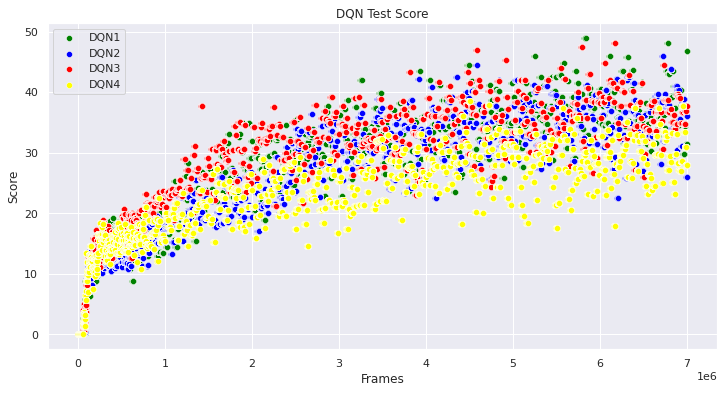
\includegraphics[scale=0.5]{DQNAgentComparison.PNG}
 \caption[width=0.7\textwidth]{DQN agent performances comparison over 7M frames. DQN1: N=200k, random experience replay selection. DQN2: N=1M, random experience replay selection. DQN3: N=200k, half prioritized experience replay selection. DQN5: N=500k, full prioritized experience replay selection.}
 \label{fig:DQNAgentComparison}
\end{figure}

Becasue of amount ot time required to train multiple agent, The traning process was then resumed until 24M frameswith DQ2 agent only.  DQN2 was chosen for two main reasons. DQN2 hiperparameters mimim the hiperparameters used by xxx which gives a clear baseline for performance comparison. Although the performances between DQN1, DQN2 and DQN3 agents do slighly vary, there is not clear cut winner. DQN4 does seem to perform the worse between the  tested configuarions. Mor details are given in section 5

\begin{figure}[H]
 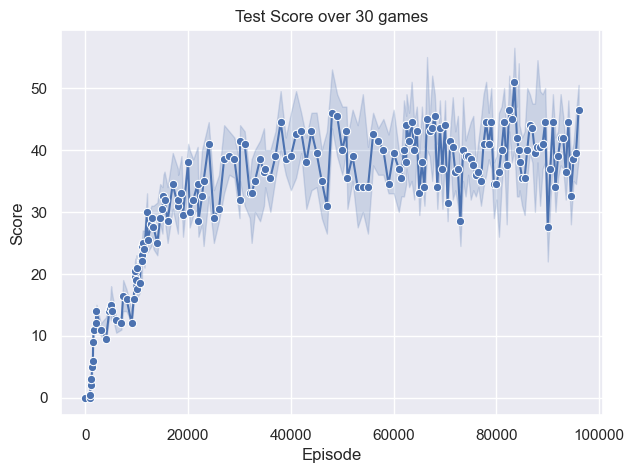
\includegraphics[scale=0.5]{DQNTestScore.PNG}
 \caption[width=0.7\textwidth]{DQN2 test score over 24M frames}
 \label{fig:DQNTestScore}
\end{figure}

Figure \ref{fig:DQNAgentComparison} and figure \ref{fig:DQNTestScore} report the test score which is the simple average over 10 games with where the exploration factor $\epsilon$  is set to 0 to obtain a deterministic policy.

\ref{fig:DQNMovAvg}  below shows the training score moving average over 10 games in blue. The green trajectory is the decaying expploration factor $\epsilon$

\begin{figure}[H]
 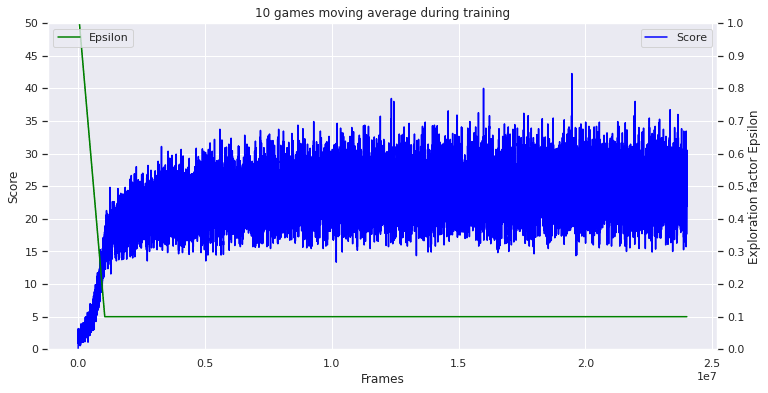
\includegraphics[scale=0.65]{DQNMovAvgTraining.PNG}
 \caption[width=0.7\textwidth]{}
 \label{fig:DQNMovAvg}
\end{figure}




\subsection{A2C (Chris)}

\begin{figure}[h]
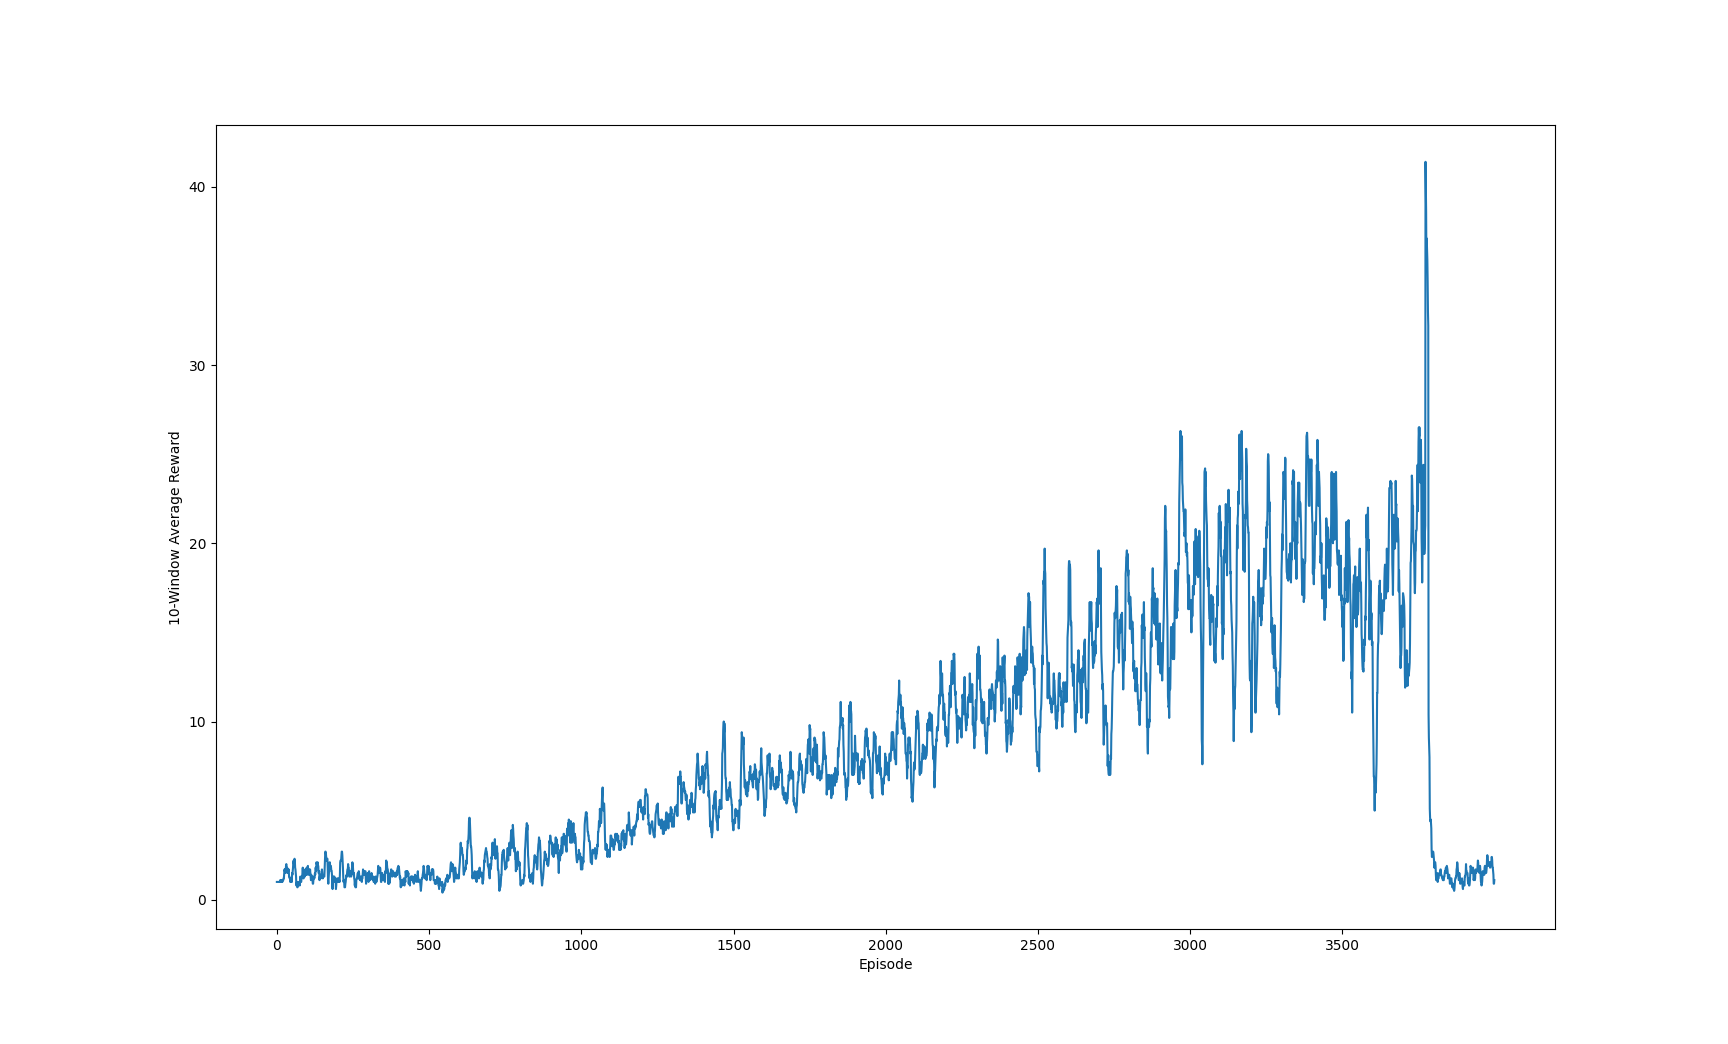
\includegraphics[scale=0.2]{A2C4000.png}
\end{figure}
\emph{Figure 4.1: 10-episode running average for Breakout A2C agent over 4000 episodes}

In the above figure, a running average of performance over a window of 10 episodes is used to provide stability in estimating agent performance. From episode 1000, the agent shows steady and notable improvement, maintaining a running average of over 10 points by episode 2500. The agent performance peaks around episode 3750 with a 10 game average of 41.4 and peak single game performance of 233. Beyond this point the agent shows evidence of overtraining. The performance significantly deteriorates to the level seen in the earliest episodes. Observing the softmax output from the actor during this period shows the agent is outputting almost the same probabilities for every state with very little change in the distribution between states or between episodes. Thus, the trained agent in the assignment video uses a weight checkpoint from earlier in the training before overtraining.


\subsection{Async Q-Learning (Peter)}

Initial results were encouraging, but the performance tended to level off quite quickly and often started to decrease.

The figure below shows a comparison of the single step Asynch Q-Learning and n-step, using n=8. The n-step approach showed a marked improvement over the single step. TODO : get better example image.

\begin{figure}[H]
\includegraphics[scale=0.4]{"async_q_learn_n_step"}
\captionof{figure}{n-step better than single step}
\end{figure}

The figures below show that the rapid initial learning slows, but with management of the epsilon value in the e-greedy policy, it does continue to improve.
TODO : Getter neater graphs with matching ranges

\begin{figure}[H]
\centering
\begin{subfigure}{0.49\textwidth}
\centering
\includegraphics[scale=0.4]{"async_q_learn_best_by_steps"}
\captionof{figure}{Reward sampled every 25 episodes}
\end{subfigure}
\begin{subfigure}{0.49\textwidth}
\centering
\includegraphics[scale=0.4]{"async_q_learn_best_epsilon_values"}
\captionof{figure}{Rewards every episode for different processes}
\end{subfigure}
\captionof{figure}{long run showing gradual improvements}
\end{figure}



\section{Discussion}
    
%An evaluation of how well you solved your chosen problem.

\subsection{DQN (Mirco)}

\subsection{A2C (Chris)}

Significant literature exists on the training of different reinforcement agents on Atari learning environments. This section compares the results obtained from this implementation with implementations in the literature along with a comparison against a baseline of performance from a professional human game tester.

\begin{table}[h!]
\centering
\begin{tabular}{|c | c | c |} 
 \hline
 Human (Baseline) & A2C Implementation & Wu et al. (2017) A2C (50mil timesteps) \\ [0.5ex] 
 \hline
 31.8 & 41.4 & 581.6  \\ 
 \hline
\end{tabular}
\end{table}
\emph{Table 5.1: Col 1- Human performance on Breakout from a profession games tester (Mnih et al., 2015). Col2 - Peak performance of A2C implementation in this assignment averaged over 10 episodes. Col3 - Performance of A2C implementation in Wu et al. (2017)  after 50 million timesteps averaged over 100 episodes}

As shown in Table 5.1, using an average over 10 games, the A2C implementation in this assignment was able to significantly outperform a professional human game tester, reaching 130.19\% of human performance. This was achieved in ~3750 episodes of training which equated to approximately 8 hours training time on CPU. As the implementation outperforms the human baseline, this indicates the agent has solved the chosen problem relatively well and achieves superhuman performance. 

However, the implementation does not come close to achieving the 100 game running average of 581.6 achieved by the A2C implementation in Wu et al. (2017). Thus, whilst the agent does solve the problem effectively enough to achieve superhuman performance, it does not match similar implementations in the literature. The agent in this implementation begins to sink into local minima significantly before the 50 million timeframe point. Interestingly, across several runs, the instability and subsequent local minima appear after a particularly high score (In this case 233), indicating that a potential cause for the deterioration in performance is a very large update to the networks that the agent is unable to properly incorporate. This suggests that, given more time and resources in the assignment, a potential route to match the high scores reached in the literature is to reduce the learning rate and training the agent for significantly longer. Unfortunately, the 50 million time-step training will require the availability of more suitable hardware than is available to the group in this assignment.

\begin{table}[h!]
\centering
\begin{tabular}{|c | c|} 
 \hline
 A2C Implementation & Wu et al. (2017) A2C (50mil timesteps) \\ [0.5ex] 
 \hline
 3774 & 14464   \\ 
 \hline
\end{tabular}
\end{table}
\emph{Table 5.2: Col 1- Episodes required for 10 episode average to surpass human performance Col2 - Episodes required for Wu et al. (2017) A2C implementation to surpass human performance over 100 episode average.}

Table 5.2 compounds the idea that the agent implemented in this paper learns quickly but that this may be the cause of the instability. Whilst the episode average windows are of different sizes, the difference number of episodes required for the A2C to surpass human performance over the chosen window is relatively large. This suggests that although the agent is unable to match the final performance of similar implementations in the literature, the agent in this implementation learns quickly. This, again, suggests that with more time and resources, a lower learning rate and a greater training time may allow this implementation to reach scores comparable to those in the literature.

\subsection{Async Q-Learning (Peter)}

As expected, the Asynch n-step Q-Learning produced better results than single step. However, they did not match the results in the time scales achieved by Mnih et al (2016). On further examination of figures published by Mnih et al (2016) the scores on the data efficiency and training time graphs show that they completed approx 25 epochs in 10 hours giving scores in excess of 250. A single epoch is 4 million frames giving 100 million frames in 10 hours. In contrast our implementation for asynch Q-Learning processed about 7.5 million frames in 10 hours, so approximately 13 times slower. 

That being the case, it gives us an expectation of 2 days processing time to acheive a score in excess of 250. The results we obtained actually compare favourably with those from Mnih et al (2016), with average scores of 25 being acheived in less than half the number of steps.

TODO : Discussion of all the different hyper parameters?

\section{Future Work}

%What other techniques can be used to improve further the performances of the 3 agents.

\subsection{A2C (Chris)}

In the A2C implementation used, the advantage function is calculated using n-step (Where n=1) returns. This only includes one step of actual rewards. Since rewards are generated from a single trajectory they tend to have high variance but are unbiased. However, the state valuation reflects all trajectories seen so far and thus has lower variance but introduces bias. As a result, the value of n controls the bias-variance tradeoff (Graesser and Loon, 2020).Thus, using 1 step returns provides us with a tradeoff of low variance but introduces significant bias through the reliance on state value.

In contrast, Generalised Advantage Estimate (GAE) overcomes the need to set n as a hyperparameter by using an exponentially-weighted average of advantages calculated with different values of n (Schulman et al., 2015). GAE provides a  method by which the low-variance, high-bias one step advantage is most heavily weighted but the lower-weighted contributions from higher values of n still contribute. By tweaking the decay rate of contribution from these higher-variance estimators with higher values of n, GAE allows a more finely controlled tradeoff between bias and variance than the hard cut-off tradeoff in n-step methods (Graesser and Loon, 2020). In comparison to the 1-step method implemented, this is likely to allow a significant reduction in bias whilst controlling the increase in variance. By testing several values for the GAE decay rate, it is possible that a lower-bias, higher-variance solution may exist that performs better than the n-step advantage implementation.

As indicated in section 5, the evidence from training time and stability in this implementation against the literature also suggests that worthy future work to extend this implementation would be to train the agent for significantly longer with a lower learning rate. However, this may require hardware above what is available to this group for the assignment.

\section{Personal Experience}
%A discussion of your personal experience with the project, such as difficulties or pleasant surprises you encountered while completing it.

\subsection{A2C (Chris)}

In the training of the A2C agent, one factor that was both a difficulty and a surprise was the sensitivity of the agent to changes in the algorithm hyperparameters. For example, the entropy weight was found to be a very important and sensitive hyperparameter. If set slightly too low the agent would revert to selecting a single action with certainty every time. If set too low the agent would not move significantly from a random sample across the four actions. However, the difference between these outcomes was often a very small change. The value used in the implementation was 0.06. A value of 0.075 was found to get stuck very close to an even weighting of actions for all states (0.25 uniformly) and a value of 0.045 would get stuck in a local minima of selecting only one action. Thus, with only a difference of 0.015 either side of the value used, the performance did not just degrade slightly but became practically untrainable. It it, however, possible that this sensitivity may have been mitigated at the cost of increased training time by reducing the learning rate of the networks.

\section*{References}

Graesser, L.H. and Keng, W.L., 2019. \emph{Foundations of deep reinforcement learning: theory and practice in Python}. First edition. Pearson addison-wesley data \& analytics series. Boston: Addison-Wesley.

Hasselt, H. van, Guez, A. and Silver, D., 2016. Deep Reinforcement Learning with Double Q-Learning. \emph{Proceedings of the AAAI Conference on Artificial Intelligence} [Online], 30(1). Available from: https://doi.org/10.1609/aaai.v30i1.10295 [Accessed 31 December 2022].

Li, S., Bing, S. and Yang, S., 2018. \emph{Distributional Advantage Actor-Critic}. [Online]. Available from: https://doi.org/10.48550/ARXIV.1806.06914 [Accessed 30 December 2022].

Machado, M.C., Bellemare, M.G., Talvitie, E., Veness, J., Hausknecht, M. and Bowling, M., 2018. Revisiting the Arcade Learning Environment: Evaluation Protocols and Open Problems for General Agents [Online]. \emph{Journal of Artificial Intelligence Research}  Available from: https://www.ijcai.org/proceedings/2018/0787.pdf  [Accessed 31 December 2022].

Mnih, V., Kavukcuoglu, K., Silver, D., Rusu, A.A., Veness, J., Bellemare, M.G., Graves, A., Riedmiller, M., Fidjeland, A.K., Ostrovski, G., Petersen, S., Beattie, C., Sadik, A., Antonoglou, I., King, H., Kumaran, D., Wierstra, D., Legg, S. and Hassabis, D., 2015. Human-level control through deep reinforcement learning. \emph{Nature} [Online], 518(7540), pp.529–533. Available from: https://doi.org/10.1038/nature14236. [Accessed 27th December 2022]

Schulman, J., Moritz, P., Levine, S., Jordan, M. and Abbeel, P., 2015. \emph{High-Dimensional Continuous Control Using Generalized Advantage Estimation}  [Online]. Available from: https://doi.org/10.48550/ARXIV.1506.02438 [Accessed 30 December 2022].

Silver, D., Huang, A., Maddison, C.J., Guez, A., Sifre, L., van den Driessche, G., Schrittwieser, J., Antonoglou, I., Panneershelvam, V., Lanctot, M., Dieleman, S., Grewe, D., Nham, J., Kalchbrenner, N., Sutskever, I., Lillicrap, T., Leach, M., Kavukcuoglu, K., Graepel, T. and Hassabis, D., 2016. Mastering the game of Go with deep neural networks and tree search. \emph{Nature} [Online], 529(7587), pp.484–489. Available from: https://doi.org/10.1038/nature16961. [Accessed 23rd December 2022]

Steinbach, A. 2018. \emph{RL introduction: simple actor-critic for continuous actions} [Online]. Medium. Available from: https://medium.com/@asteinbach/rl-introduction-simple-actor-critic-for-continuous-actions-4e22afb712 [Accessed 22nd December 2022]

Sutton, R.S. and Barto, A.G., 2018. \emph{Reinforcement learning: an introduction}. Second edition. Adaptive computation and machine learning series. Cambridge, Massachusetts: The MIT Press.

Williams, R.J. and Peng, J., 1991. Function Optimization using Connectionist Reinforcement Learning Algorithms. \emph{Connection Science} [Online], 3(3), pp.241–268. Available from: https://doi.org/10.1080/09540099108946587. [Accessed 27th December 2022]

Wu, Y., Mansimov, E., Liao, S., Grosse, R. and Ba, J., 2017. \emph{Scalable trust-region method for deep reinforcement learning using Kronecker-factored approximation} [Online]. Available from: https://doi.org/10.48550/ARXIV.1708.05144 [Accessed 30 December 2022].

Wang, M. 2021. \emph{Advantage Actor Critic Tutorial: minA2C} [Online]. Medium. Available from: https://towardsdatascience.com/advantage-actor-critic-tutorial-mina2c-7a3249962fc8 [Accessed 24th December 2022].

Wu, Y., Mansimov, E., Liao, S., Radford, A. and Schulman, J., 2017. \emph{OpenAI Baselines: ACKTR \& A2C} [Online].OpenAI. Available from: https://openai.com/blog/baselines-acktr-a2c/ [Accessed 30 December 2022].

Yoon, C. 2019. \emph{Understanding Actor Critic Methods and A2C} [Online]. Towards Data Science. Available from: https://towardsdatascience.com/understanding-actor-critic-methods-931b97b6df3f [Accessed 24th December 2022]


\small

Mnih, V., et al., 2016. Asynchronous Methods for Deep Reinforcement Learning. ArXiv, [Online] 1602.01783.
Available from: \url{https://arxiv.org/pdf/1602.01783.pdf} [Accessed 28 Dec 2022]

\normalsize
\newpage
\section*{Appendices}
%If you have additional content that you would like to include in the appendices, please do so here.
%There is no limit to the length of your appendices, but we are not obliged to read them in their entirety while marking. The main body of your report should contain all essential information, and content in the appendices should be clearly referenced where it's needed elsewhere.
\subsection*{Appendix A: DQN pseudo-code}
\label{dqn_pseudo}
Taken from the course notes.
\begin{algorithmic}[1]
\State Initialise replay memory $D$ to capacity $N$
\State Initialise action-value network $\hat{q}_{1}$ with parameters $\boldsymbol{\theta}_{1} \in \mathbb{R}^{d}$ arbitrarily
\State Initialise target action-value network $\hat{q}_{2}$ with parameters $\boldsymbol{\theta}_{2}=\boldsymbol{\theta}_{1}$
\For{each episode}
    \State $\text{Initialise } S$
    \For{for each step of episode}
        \State Choose action $A$ in state $S$ using policy derived from  $\hat{q}_{1}\left(S, \cdot, \theta_{1}\right)$
        \State Take action $A$ observe reward $R$ and next-state $S^{\prime}$
        \State Store transition $\left(S, A, R, S^{\prime}\right)$ in $D$
        \For{each transition $\left(S_{j}, A_{j}, R_{j}, S_{j}^{\prime}\right)$ in minibatch sampled from $D$}
            \State $y= \begin{cases}R_{j} & \text { if } S_{j}^{\prime} \text { is terminal } \\ R_{j}+\gamma \max _{a^{\prime}} \hat{q}_{2}\left(S_{j}^{\prime}, a^{\prime}, \boldsymbol{\theta}_{2}\right) & \text { otherwise }\end{cases}$
            \State $\hat{y}=\hat{q}_{1}\left(S_{j}, A_{j}, \boldsymbol{\theta}_{1}\right)$
            \State Perform gradient descent step $\nabla_{\theta_{1}} L_{\delta}(y, \hat{y})$
        \EndFor
    \State Every $C$ time-steps, update $\boldsymbol{\theta}_{2}=\boldsymbol{\theta}_{1}$
    \EndFor
\EndFor
\end{algorithmic}

\subsection*{Appendix B: TD Advantage Actor Critic (A2C) pseudo-code}
\label{async_a2c_pseudo}

From Steinbach (2018)

\begin{algorithmic}[1]
\State Randomly initialise critic network $V^{U}_{\pi}(s)$ and actor network $\pi^{\theta}(s)$ with weights U and $\theta$
\State Initialise environment $E$
\For{episode = 1, M}
\State Receive initial observation state $s_{0}$ from $E$
\For{t=0, T}
\State Sample action $a_{t} \sim \pi(a | \mu, \sigma) = \mathcal{N}(a | \mu, \sigma)$ according to current policy
\State Execute action $a_{t}$ and observe reward $r$ and next state $s_{t+1}$ from $E$
\State Set TD target $y_{t} = r + \gamma \cdot V^{U}_{\pi}(s_{t+1})$
\State Update critic by minimising loss: $\delta_{t} = (y_{t} - V^{U}_{\pi}(s))^{2}$
\State Update actor by minimising loss: $Loss = -\log({\mathcal{N}(a | \mu(s_{t}), \sigma(s_{t}))}) \cdot \delta_{t}$
\State Update $s_{t} {\leftarrow} s_{t+1}$
\EndFor
\EndFor
\end{algorithmic}


\subsection*{Appendix C: Async Q-Learning pseudo-code}
\label{async_q_pseudo}

From Mnih et al (2016)

\begin{algorithmic}[1]
\State \textit{// Assume global shared  $\theta$, $\theta^{-}$, and counter $T = 0$}
\State Initialise thread step counter $t \gets 0$
\State Initialise target network weights $\theta^{-} \gets \theta$
\State Initialise network gradients $d\theta \gets 0$
\State Get initial stats $s$
\While{$T <= T_{\max}$}
    \State Take action $a$ with $\epsilon$-greedy policy based on $Q\left(s,a;\theta\right)$
    \State Receive new state $s^{\prime}$ and reward $r$
    \State $y= \begin{cases}r & \text { for terminal } s^{\prime} \\ r + \gamma \max _{a^{\prime}} Q\left(s^{\prime}, a^{\prime}, \theta^{-}\right) & \text { for non terminal } s^{\prime}\end{cases}$
    \State Accumulate gradients wrt $\theta$: $d\theta \gets d\theta + \frac{\delta\left( y-Q\left(s, a, \theta\right)\right)^{2}}{\delta\theta}$
    \State $s = s^{\prime}$
    \State $T \gets T + 1$ and $t \gets t + 1$
    \If{$T$ mod $I_{target} == 0$}
        \State Update the target network $\theta^{-} \gets \theta$
    \EndIf
    \If{$t$ mod $I_{AsyncUpdate} == 0$ or $s$ is terminal}
        \State Perform asynchronous update ot $\theta$ using $d\theta$
        \State Clear gradients $d\theta \gets 0$
    \EndIf
\EndWhile

\end{algorithmic}

\subsection*{Appendix D: Async n-step Q-Learning pseudo-code}
\label{async_q_n_step_pseudo}

From Mnih et al (2016)

\begin{algorithmic}[1]
\State \textit{// Assume global shared  $\theta$, $\theta^{-}$, and counter $T = 0$}
\State Initialise thread step counter $t \gets 0$
\State Initialise target network weights $\theta^{-} \gets \theta$
\State Initialise network gradients $d\theta \gets 0$
\State Initialise thread-specific parameters $\theta^\prime \gets \theta$
\State Get initial stats $s$
\While{$T <= T_{\max}$}
    \State Clear gradients $d\theta \gets 0$
    \State Synchronize thread-specific parameters $\theta^\prime \gets \theta$
    \State $t_{start} = t$
    \State Get state $s_t$
    \While{not terminal $s_t$ and $t-t_{start}<t_{max}$}
        \State Take action $a_t$ with $\epsilon$-greedy policy based on $Q\left(s_t,a;\theta^\prime\right)$
        \State Receive new state $s_{t+1}$ and reward $r_t$
        \State $t \gets t + 1$
        \State $T \gets T + 1$
    \EndWhile
    \State $R= \begin{cases}0 & \text { for terminal } s_t \\ \max _{a} Q\left(s_t, a, \theta^{-}\right) & \text { for non terminal } s_t\end{cases}$
    \For{$i \in \{t-1,...,t_{start}\}$}
        \State $R \gets r_i + \gamma R$
        \State Accumulate gradients wrt $\theta^\prime$: $d\theta \gets d\theta + \frac{\delta\left( y-Q\left(s, a, \theta\prime\right)\right)^{2}}{\delta\theta\prime}$
    \EndFor
    \State Perform asynchronous update ot $\theta$ using $d\theta$
    \If{$T$ mod $I_{target} == 0$}
        \State Update the target network $\theta^{-} \gets \theta$
    \EndIf
\EndWhile

\end{algorithmic}


\subsection*{Appendix E: }

\end{document}
